%!TEX root = main.tex

\section{Introduction} \label{sec:intro}

% autonomous vehicle common experience
Autonomous vehicles use onboard sensors to perceive their surroundings, and use the data to make decisions about where it is safe to drive.
Today's research vehicles typically rely on Lidar and cameras as the main sensors, as these provide information about where/what obstacles are, and can help the vehicle maintain safe position in its lane and with respect to obstacles.
In addition to static obstacles, vehicles interact with pedestrians in a variety of environments: people in crosswalks, jaywalkers, kids running across neighborhood streets.
A campus shuttle could even drive on sidewalks among pedestrians, so the vehicle would be interacting with pedestrians almost all the time.
These regular interactions mean the vehicle must be able to predict pedestrians' next moves in order to maintain safety.

% what is challenging about pedestrians/what info do we have
Pedestrian motion prediction is difficult because people often behave very unexpectedly.
Humans use many strategies to predict pedestrian intent while driving, such as body language, eye contact, and other non-verbal cues between human driver and human pedestrian, but autonomous vehicles can't easily communicate or read these signals.
The information from sensors is typically fused: Lidar is used to measure the pedestrian position, and the camera is used to label the particular obstacle as a pedestrian.
Therefore the only measurements collected are position over time (from which velocity can also be computed).

\begin{figure}
\centering
\begin{subfigure}{.25\textwidth}
  \centering
  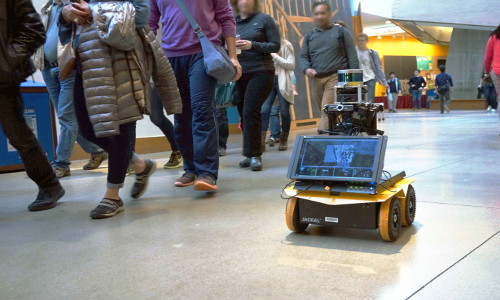
\includegraphics[width=.9\linewidth]{figures/rover_d}
  \caption{Ground robot in Stata}
  \label{fig:jackal}
\end{subfigure}%
\begin{subfigure}{.25\textwidth}
  \centering
  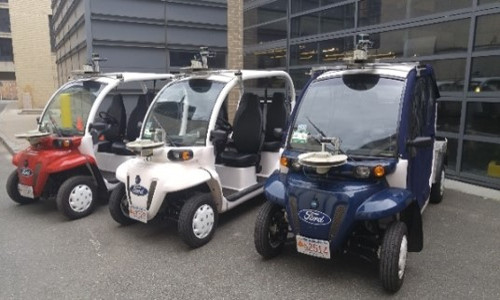
\includegraphics[width=.9\linewidth]{figures/mod_testbed}
  \caption{Golf carts (MIT MoD fleet)}
  \label{fig:golf_carts}
\end{subfigure}
\caption{Many types of autonomous vehicles operate among pedestrians and must account for pedestrian motion in the vehicle motion planning algorithms.}
\label{fig:vehicles}
\end{figure}

This project uses a dataset collected on MIT's campus over several months by three golf cart shuttles providing Mobility on Demand service to students, while simultaneously collecting pedestrian trajectory data to optimize vehicle routing strategy.
The dataset contains about 65,000 pedestrian trajectories as well as the vehicles' trajectories, all in a global frame across the MIT campus.

% what has been done in research?
We omit a thorough literature review section for the sake of brevity -- relevant works that are specifically used in the project are cited throughout.

% what is our goal/how do we evaluate?
The objective of this project is to develop a classifier that can determine whether a person will step in front of a vehicle, based on a few seconds of their trajectory.
We use a portion of our data set to train different classifiers, optimize hyperparameters with a separate portion, and evaluate performance with yet another portion.
This classifier could be a useful component of an autonomous vehicle, or part of an active safety feature on a human-driven vehicle that could take over in case the driver does not see a pedestrian in time.

% what are contributions
The main contributions of this work are 
(i) an SVM classifier for predicting when pedestrians will step in front of a vehicle, (ii) a classifier using LSTMs for that same objective, and (iii) initial results for pedestrian motion prediction using LSTMs.











